\section{Problema dei 3 corpi: perturbazioni e problema ristretto}

\begin{frame}{Problema dei 3 corpi. Problema ristretto.}

\begin{itemize}
\item Terra-Sole-Giove
\item Terra-Sole-Luna
\item Giove-Saturno-Sole
\end{itemize}

\begin{block}{Problema ristretto}

\begin{columns}

\begin{column}{0.5\textwidth}

\begin{itemize}
\item Un corpa ha massa trascurabile risp. altri 2
\item Moto piano
\item Distanza tra i 2 primari costante
\end{itemize}

\end{column}


\begin{column}{0.5\textwidth}

Sole-Giove-Asteroide

Terra-Luna-Satellite artificiale

\begin{figure}

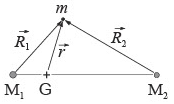
\includegraphics[keepaspectratio,width=0.6\textwidth]{3Brestrict}

\end{figure}

\end{column}

\end{columns}

\end{block}

\end{frame}

\begin{wordonframe}{Problema dei 3 corpi e problema ristretto}

\begin{align*}
&n_0a_0^3=G(M_1+M_2)
\end{align*}

Masse: $M_M\approx0.012$, $M_E=1$, $M_S\approx98$, $M_J\approx318$, $\msun{}\approx\num{3.3e5}$



Nel sistema Terra-Luna-Sole l'attrazione del Sole sulla Luna \'e una perturbazione nel sistema non inerziale che orbita attorno al Sole. 


\end{wordonframe}


\begin{frame}{Riferimento rotante}

\begin{columns}

\begin{column}{0.5\textwidth}

\begin{block}{Forza di Coriolis}
\begin{equation*}
\vec{f}_{cor}=-2m\vec{n}_0\wedge\dvec{r}
\end{equation*}
Lavoro nullo: ortogonale alla velocit\'a.

\end{block}

\end{column}

\begin{column}{0.5\textwidth}

\begin{block}{Forza centrifuga}
\begin{equation*}
\vec{f}_{cen}=-\nabla(-\frac{1}{2}m|\vec{n}_0\wedge\vec{r}|^2)
\end{equation*}
\'E conservativa.

\end{block}

\end{column}

\end{columns}

\begin{block}{Integrale di Jacobi}

\begin{equation*}
E=\frac{1}{2}m|\dvec{r}|^2-\frac{GM_1m}{R_1}-\frac{GM_2m}{R_2}-\frac{1}{2}m|\vec{n}_0\wedge\vec{r}|^2
\end{equation*}

\end{block}


\end{frame}

\begin{wordonframe}{Sistemi non inerziali, energia, forze conservative}

\begin{align*}
m\ddvec{x}=\vec{F}-m\dvec{\Omega}\wedge\vec{x}-2m\vec{\Omega}\wedge\dvec{x}-m\vec{\Omega}\wedge(\vec{\Omega}\wedge\vec{x})
\end{align*}

\end{wordonframe}

\begin{frame}{Regioni energeticamente permesse e punti di equilibrio}

\begin{columns}

\begin{column}{0.43\textwidth}

\begin{block}{Punti di equilibrio}

\begin{align*}
&\frac{1}{m}\nabla V=0\\
&=-n_0^2\vec{r}+\frac{GM_1}{R_1^3}\vec{R}_1+\frac{GM_2}{R_2^3}\vec{R}_2\\
&\vec{R}_1\nparallel\vec{R}_2:\\
&\vec{R}_1=\vec{R}_2=a_0 \Rightarrow L_4, L_5
\end{align*}

\end{block}


\end{column}

\begin{column}{0.57\textwidth}

\begin{block}{Superfici a velocit\'a nulla (di Hill)}

\begin{figure}[!t]

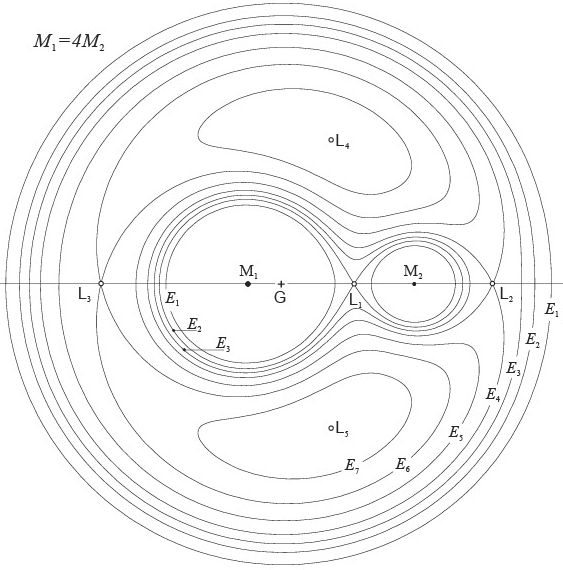
\includegraphics[keepaspectratio,width=0.9\textwidth]{hillzero}

\end{figure}

\end{block}

\end{column}

\end{columns}

Troiani

\end{frame}

\begin{wordonframe}{Superficie di Hill e punti Lagrangiani}

$L_1$, $L_2$, $L_3$: equilibrio instabile.

$L_4$, $L_5$: equilibrio stabile per $\frac{M_1}{M_2}>25$.

Oscillazioni attorno ai punti di equilibrio

\end{wordonframe}

\begin{frame}{Criterio Tisserand}

\begin{itemize}
\item $M_1\gg M_2$
\item $R_2$ a grandi distanze (cometa distante da Giove)
\end{itemize}

\begin{block}{Relazione di Tisserand}

\begin{equation*}
\frac{1}{2a}+\sqrt{\frac{a(1-e^2)}{a_0^3}}\cos{i}=const
\end{equation*}

\end{block}

\begin{block}{Velocit\'a relativa}

\begin{align*}
&v_{rel}=\frac{G\msun{}(3-T)}{a_0}\quad T=\frac{a_0}{2a}+\sqrt{\frac{a(1-e^2)}{a_0}}\cos{i}
\end{align*}

\end{block}

\end{frame}

\begin{wordonframe}{Criterio Tisserand}

a: semiasse cometa, $a_0$: semi-asse J, e,i eccentricit\'a inclinazione cometa

L'espressione connette gli elementi orbitali di una cometa (lontano da Giove) a pasaggi successivi.

Velocit\'a nel riferimento inerziale: $\TDy{t}{\vec{r}}=\dvec{r}+\vec{n}_0\wedge\vec{r}$.

\begin{align*}
&\vec{R}_1=\vec{r}+\frac{M_1}{M_1+M_2}\vec{a}_0\Rightarrow\TDy{t}{\vec{r}}=\TDy{t}{\vec{R}_1}-\frac{M_1}{M_1+M_2}\vec{n}_0\wedge\vec{a}_0\\
&E=E_1+c\\
&E_1=\frac{1}{2}|\TDy{t}{\vec{R}_1}|^2-\frac{GM_1}{R_1}-\frac{GM_2}{R_2}-\vec{n}_0\cdot\vec{R}_1\wedge\TDy{t}{\vec{R}_1}+\frac{M_1}{M_1+M_2}n_0^2\vec{a}_0\cdot\vec{R}_1
\end{align*}

Gli ultimi 2 termini descrivono variazione energetiche dovute ad azione cometa su Sole e Jupiter; in approx $M_1\gg M_2$: $E_1\approx E_c-\vec{n}_0\cdot\vec{J}_c$

\end{wordonframe}

\begin{wordonframe}{Velocit\'a relativa J-comet}
($r\approx a_G$)
\begin{align*}
&v_{\theta}=\frac{h}{a_G}=\sqrt{\frac{G\msun{}}{a_G}}\sqrt{\frac{a_c(1-e_c^2)}{a_G}}\\
&v^2=G\msun{}[\frac{2}{a_G}-\frac{1}{a_c}]\\
&v_{rev}=v^2-v_{\theta}^2=\frac{G\msun{}}{a_G}[3-\frac{a_G}{a_c}-2\cos{i}\sqrt{(1-e_c^2)\frac{a_c}{a_G}}]
\end{align*}

\end{wordonframe}

\begin{frame}{Problema 3 corpi ristretto: integrali primi}

\begin{columns}[T]

\begin{column}{0.5\textwidth}

\begin{block}{sistema a 2 gradi di libert\'a}

Sistema a 2 gradi di libert\'a ha 3 integrali primi.

\end{block}

\end{column}

\begin{column}{0.5\textwidth}

\begin{block}{Integrali primi uniformi}
Integrali primi continui
\end{block}

\begin{block}{Analiticit\'a}

$\epsilon=\frac{M_2}{M_1}$ ($\epsilon=0$: problema a 2 corpi)

\end{block}

\end{column}

\end{columns}

\begin{block}{Poincar\'e (1890)}

Il problema dei 3 corpi ristretto ha solo l'integrale di Jacobi come integrale uniforme e analitico in $\epsilon$.

\end{block}

Il problema a 3 corpi (ristretto non \'e integrabile)

\begin{block}{Comportamento caotico}

\begin{columns}[T]

\begin{column}{0.5\textwidth}
Conoscenza condizioni iniziali con precisione finita
\end{column}

\begin{column}{0.5\textwidth}
Divergenza esponenziale delle traiettorie nello spazio delle fasi.
\end{column}

\end{columns}

\end{block}

\end{frame}

\begin{wordonframe}{Integrali primi}

\begin{columns}[T]
\begin{column}{0.5\textwidth}
\begin{align*}
&x(0),y(0)\\
&\dot{x}(0),\dot{y}(0)
\end{align*}
\end{column}

\begin{column}{0.5\textwidth}
Soluzione equazione del moto: Curva nello spazio delle fasi $F(x,y)=c$.
\end{column}

\end{columns}

Sistema integrabile a n-dof: n variabili angolo $\phi_i$ (variano linearmente nel tempo), n variabili azione (costanti del moto)

\begin{block}{Liuville-Arnol'd}
Una traiettoria di fase \'e densa nel suo toro n-dimensionale
\end{block}

\end{wordonframe}


\begin{frame}{Problema a 3 corpi: disuguaglianza di Easton}

Sistema legato di n punti materiale con baricentro fermo.

\begin{columns}[T]

\begin{column}{0.5\textwidth}
\begin{equation*}
IV^2\geq2|E|J^2
\end{equation*}
\end{column}

\begin{column}{0.5\textwidth}
$2|E|J^2$: costante del moto (Integrale di Zare).

$IV^2$: dipende dalla configurazione del sistema e non dalla velocit\'a

\end{column}

\end{columns}


\end{frame}
